%!TEX root = ../thesis.tex
%*******************************************************************************
%****************************** Third Chapter **********************************
%*******************************************************************************
\chapter{Toward Culturally Competent Robotic Architectures }
\label{ch5}

% **************************** Define Graphics Path **************************
\ifpdf
    \graphicspath{{Chapter5/Figs/Raster/}{Chapter5/Figs/PDF/}{Chapter5/Figs/}}
\else
    \graphicspath{{Chapter5/Figs/Vector/}{Chapter5/Figs/}}
\fi

The second part of this thesis proposes a novel framework for implementing cultural competence in SRs.
%\color{red} Nell'introduzione avevi parlato di due parti, prima con due 
%\color{black}
It also presents the experiments designed and conducted during my research stay at ETH Zurich, in which a possible implementation of the proposed framework was deployed on the Pepper SR.

This chapter presents the proposed framework and its constituent components. 
In addition, it presents the implementation evaluated on the Pepper SR.
The chapter also introduces the cultural dimensions used to characterize participants and the measures adopted to assess the cultural competence exhibited by the robot during the experiments. 

\section{System Architecture}

The proposed architectural framework is based on the premise that SRs require the ability to represent, reason about, and act upon environmental knowledge~\citep{SocialRobotics}, which is inherently influenced by cultural factors. 
To support this capability, the system must acquire raw sensory data, abstract these inputs into semantic representations, perform high-level reasoning, and subsequently generate contextually appropriate behavioral responses through its actuators. 
The recent emergence of LLM-based agents has enabled traditional robotic architectures to be extended with flexible reasoning components that can dynamically adapt their behavior to the interaction context. 
This abstraction enables cultural competence to be incorporated at different levels of granularity throughout the system pipeline. 
The proposed architecture is intended to encompass all such levels; consequently, the schema presented in Figure~\ref{ch5:fig:CCF} is deliberately abstract and general in order to remain applicable across a wide range of robotic platforms, implementations, and social contexts.
We remark here, that cultural competence is the ability of a system to adapt to different cultural contexts.
A component is therefore culturally competent, when it can embed cultural parameters that can vary depending on the context and still works properly.

\begin{figure}
    \centering
    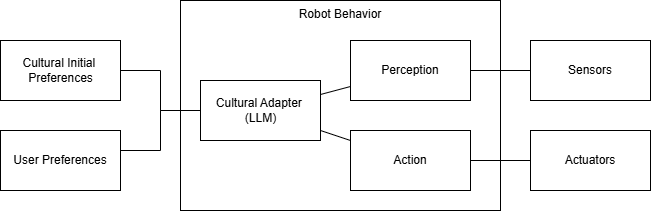
\includegraphics[width=\linewidth]{Figs/architecture.drawio.png}
    \caption{General Schema for Culturally Competent SRs.}
    \label{ch5:fig:CCF}
\end{figure}

The architecture can be described from a temporal interaction perspective as follows:
\begin{itemize}
    \item Sensors Component: captures raw environmental signals and converts them into low-level digital representations (e.g., audio sampled as a waveform);
    \item Perception Component: transforms low-level sensor data into higher-level representations (e.g., speech signals converted into text via a Speech-to-Text (STT) system);
    \item Cultural Adapter Component: reasons over high-level representations, initial cultural priors, and learned user preferences to adapt both perception and action parameters. For example, if the user requests a language change, the system updates the user preference model, reconfigures the perception pipeline (e.g., STT language settings), and adapts the action pipeline to generate output in the target language using Text-to-Speech (TTS);
    \item Cultural Initial Preferences and User Preferences Components: These components act as memory repositories. The Cultural Initial Preferencescomponent stores the user's national culture or initial preference profile, while the User Preferences component stores the preferences learned and updated by the Cultural Adapter component. These preferences are represented as cultural parameters that influence the entire processing pipeline.
    \item Action Component: converts high-level system commands into modality-specific outputs (e.g., text into speech synthesis commands using TTS);
    \item Actuators Component: execute low-level control signals to produce physical effects in the environment (e.g., rendering synthesized audio through speakers).
\end{itemize}

Current SR architectures often rely on predefined cultural models and fixed national-level parameters. 
While such approaches can capture broad cultural tendencies, they typically provide limited flexibility in the acquisition and manipulation of cultural knowledge~\citep{akinade2023culturally}. 
Consequently, they are not designed to take into account intra-cultural heterogeneity and individual preferences that diverge from the statistical norm of a cultural group. 
For example, in many regions users may prefer regional dialects or minority languages over the official national language, a nuance that is difficult to represent through monolithic cultural models. 
Recent advances in LLMs offer a potential solution to these limitations. 
Owing to their large-scale pre-training on diverse and heterogeneous corpora, LLMs can capture complex cultural distributions and implicitly encode both dominant cultural patterns and subcultural variations. 
Furthermore, their ability to interact with external tools and knowledge sources enables them to function as adaptive reasoning components within larger robotic systems.

The proposed framework is based on two premises. 
First, cultural domain knowledge is partially encoded within the latent representations of LLMs. 
Second, knowledge-injection techniques such as Retrieval-Augmented Generation (RAG)\cite{lewis2020retrieval} allow LLMs to access external and continuously updatable sources of information. 
%\color{red} Citazione mancante \color{black} 
In this context, RAG is not employed solely to retrieve static cultural priors. 
Rather, the combination of implicit cultural knowledge and retrieved information enables the LLM to dynamically configure the constituent modules of the robotic architecture, including user preference modeling, perception, and action generation. 
Compared with alternatives such as fine-tuning, RAG is particularly suitable due to the scarcity of culturally annotated data, its lower computational requirements, and its ability to incorporate new information without retraining.

An illustrative example of this adaptive capability is language selection during interaction. 
In human-to-human communication, individuals may default to a locally dominant language, yet communication often becomes more effective when interlocutors switch to a mutually intelligible language. 
Conversely, when both individuals share a native language, interaction may be equally or more effective in that language. 
Accordingly, the proposed framework treats language as a dynamic cultural variable whose value should be inferred and continuously refined according to the communicative needs and preferences of the user. 
More broadly, the framework assumes that the user is the most reliable source of information regarding their own cultural characteristics. 
Through natural language dialogue, the system can directly query users, acquire personalized cultural information, and iteratively update its representation of relevant cultural variables over time.

We propose two conceptual approaches with respect to classical frameworks. The first is the Foreknowledge (F) approach, in which fixed cultural parameters are provided to the system and augmented by LLM capabilities. In this setting, the robot is initialized with national-level cultural priors but does not update them during interaction.

The second approach, the Adaptation (A) strategy, extends the F approach by introducing a dynamic adaptation mechanism. In this configuration, the LLM is used to update the memory bank and modify cultural parameters based on interaction data. As a result, the system progressively adapts its behavior to align with individual user preferences.

Both approaches are evaluated against a Baseline (B) condition in which cultural factors are not explicitly modeled. A completely culture-neutral system is not strictly achievable, since any artifact necessarily reflects design assumptions shaped by its creators. However, for the purposes of this work, the baseline refers to a system that does not explicitly embed language- or culture-specific parameters, but instead relies on default behavior derived from general population-level assumptions.

Language provides a concrete example. If language is treated as a cultural parameter and Italian culture is used as the reference context, a baseline system may default to English due to its widespread international use. In contrast, the F approach initializes interaction in Italian, reflecting linguistic norms associated with the target cultural context. The A approach introduces an additional layer of personalization: when interacting with individuals belonging to minority populations in Italy, such as tourists, expatriates, or exchange students, the system may infer a preference for English and switch accordingly.

%\color{red} Per far vedere che è un'idea generale, metterei anche un altro esempio, sottolineando che non è stato implementato. Oppure quello prossemico (implementato) e poi un esempio non implementato.
%\color{black}
Another example could be interpersonal distance. Interpersonal distance depends on context and on culture. Some culture might prefer being closer, some further. In this case, a baseline system might just perform an overall average of all the samples collected. F approach would initialize the system depending on the clusters. Italians might have a tendency of preferring a certain distance. The A approach would optimize that value asking for references to the user. 
%\color{blue}
Both examples have been included in the implementation. 
More examples could be found, such as dinner time or food preferences, which however have not been implemented in this thesis.
%\color{black}
\section{System Implementation}
\label{sec:sys_impl}

The system is implemented on the Pepper SR, a semi-humanoid platform originally developed by Aldebaran Robotics and later acquired by SoftBank Robotics Europe. Pepper is designed for human–robot interaction, supporting speech-based communication, basic autonomous navigation, and expressive non-verbal behaviors. Figure~\ref{ch6:fig:pepper} shows the robot used in this study.
%\color{red} Foto robot intero se vuoi far vedere come è fatto, e più piccola.
%\color{black}

\begin{figure}
\centering
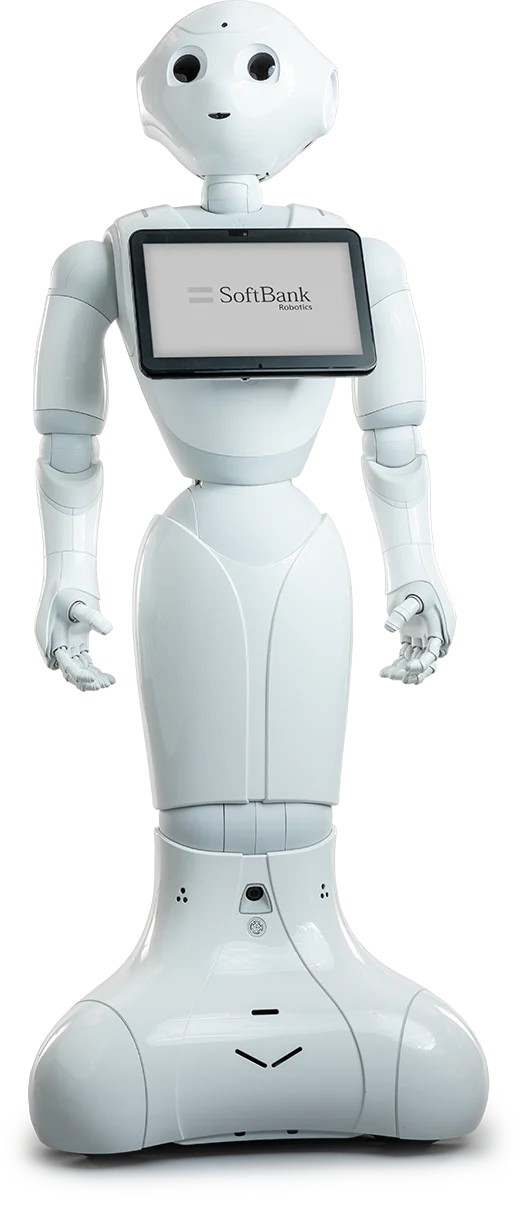
\includegraphics[width=0.3\linewidth]{Chapter5/Figs/SBR_Pepper-Hero_FullRobot.jpg}
\caption{Pepper social robot used in this study.}
\label{ch6:fig:pepper}
\end{figure}

The version used in this work is Pepper 1.8. The platform is programmable via an Android-based SDK, allowing development through Android Studio using Kotlin and Java. The SDK exposes APIs for speech synthesis and recognition, navigation, and basic gesture-based interaction, including head and torso movements that simulate social engagement cues.

To support the computational requirements of the proposed architecture, the system adopts a client--server configuration. Due to the limitations of Pepper's onboard hardware, low-level functions such as motor control, localization, and sensor acquisition are executed directly on the robot, while high-level modules—including dialogue management, cultural adaptation, and path planning—run on an external server. The server is hosted on a Windows 11 workstation equipped with an Intel Core i7-13620H CPU (10 cores, 16 threads), 16 GB DDR5 RAM (5200 MT/s), and an NVIDIA GeForce RTX 4060 Laptop GPU with 8 GB GDDR6 VRAM.

%Having described the system implementation \color{red} Non mi sembra che tu abbia descritto il system implementation. Non dici nulla di come implementi il sistema che nelle tre versioni baseline, F e A. Io terrei solo il paragrafo che segue e poi mi fermerei. I dettagli del setup sperimentale vengono dopo.
%\color{black}, the following section presents the experimental scenario used to evaluate the proposed framework. 

The selected application domain is home assistance, a context in which culturally adaptive interaction is particularly relevant. In this scenario, Pepper must navigate within an indoor environment while maintaining a conversation with the user. This setting provides opportunities to apply the cultural adaptation module at multiple levels of the system, including language selection, communication style, and proxemic behavior during navigation.

The experimental setup consists of a controlled indoor environment in which the robot navigates while interacting with a stationary participant. Pepper moves from point A to point B and back while conversing with the participant, who remains standing in a fixed position. Points A and B correspond to opposite corners of a approximately $3 \times 3$ m room, while the human is positioned near a different corner of the same environment. This configuration allows the robot to generate different navigation paths while accounting for proxemic constraints.
Figure~\ref{fig:upper_view} represents an upper map of the room with the robots trajectory from A to B and humans position.

\begin{figure}[ht]
    \centering
    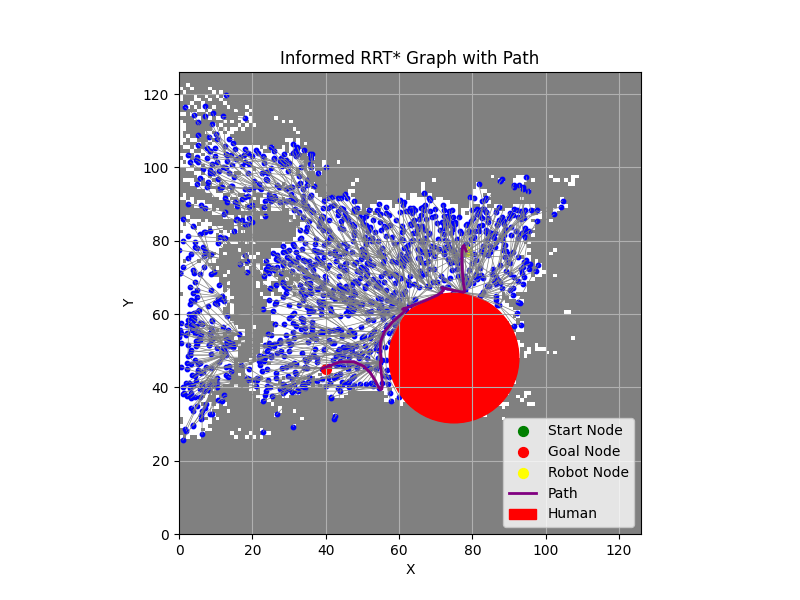
\includegraphics[width=\linewidth, trim={0 0 0 2.0cm}, clip]{Figs/40_45_to_80_80_prox=17.68_back=True.png}
    \caption{Map of the room generated by the SLAM algorithm of Pepper. Red piece-wise line is an example of the trajectory generated by the path planning algorithm of the robot from point A to point B. The red bubble is the area of proximity to human in which the robot must not enter, while its center is the human position.}
    \label{fig:upper_view}
\end{figure}

%\color{red} Mettere figura dall'alto con i punti della stanza, dove è il robot, dove è l'umano.
%\color{black}
Although intentionally simplified, the scenario preserves the key components required to evaluate the proposed framework, including culturally conditioned dialogue, perception, and navigation behaviors. At the same time, the controlled nature of the environment limits potential confounding factors and facilitates the analysis of the cultural adaptation mechanisms under investigation.

\subsection{Cultural Parameters}
\label{ch6:sec:cultural_parameters}

The proposed framework encodes cultural information as a structured set of parameters that jointly condition high-level decision-making and low-level interaction behavior. These parameters are represented through two complementary mechanisms: Cultural Initial Preferences, which define prior assumptions at system initialization, and User Preferences, which are iteratively updated during interaction. Together, they influence perception, dialogue, and action modules in a unified manner. The selected parameter space is grounded in the interaction modalities relevant to the experimental scenario, namely language, communication style, and proxemics.

Language is treated as a primary interface variable for human–robot communication. It determines the operational language used by STT, TTS, and language generation components within the dialogue system. Rather than assuming a fixed mapping between language and nationality, language is modeled as an individual-level preference that may vary independently of cultural affiliation. Empirical evidence suggests that linguistic preferences are context-dependent and cannot be reliably inferred from national identity alone, as users may select dialects, minority languages, or non-native languages depending on situational and personal factors. In the proposed system, language selection conditions all linguistic modules, ensuring consistency across STT, TTS, and LLM-based response generation.

Communication style defines how information is linguistically structured during interaction. It is operationalized using the high-context versus low-context distinction from cultural communication theory, where high-context communication relies on implicit meaning and contextual cues, whereas low-context communication emphasizes explicit and direct expression. This parameter modulates the prompting strategy of the language model, influencing response verbosity, explicitness, and interactional framing. As such, it ensures that generated outputs remain aligned with the selected communicative profile.

Proxemics models interpersonal distance regulation during human–robot interaction. It is implemented as a preferred interaction distance $D_{pref}$ associated with each cultural profile. This parameter directly influences the navigation module by shaping the cost function used in path planning, penalizing trajectories that violate socially acceptable distances. Given the variability of proxemic preferences across individuals and contexts, baseline values are derived from prior literature and subsequently refined through a preliminary empirical study conducted for the experimental setup.

All cultural parameters are integrated into a unified system representation that links dialogue and navigation modules. While language and communication style primarily condition the dialogue system and language model behavior, proxemics directly affects motion planning. Importantly, all parameters remain dynamically adjustable during interaction and can be updated when user-specific preferences are inferred while performing A paradigm, while they are static otherwise. This design frames cultural adaptation as a system-level property rather than a module-specific feature, ensuring coherence between linguistic behavior and physical navigation.

\subsection{Conversation}
\label{ch6:sec:conversation}

The dialogue management system operates on the client-side and governs the linguistic behavior of the robot during human--robot interaction. It conditions LLM outputs according to experimental constraints, cultural parameters, and interaction state. The system is implemented as a rule-conditioned interface using the Ollama framework~\footnote{\href{https://ollama.com/}{https://ollama.com/}}, enabling local deployment of a Llama 3.1 8B model.
The LLM is deployed locally and selected for computational efficiency, multilingual capability, and long-context support (up to 128k tokens). On the robot, STT and TTS modules are dynamically updated in the A condition to maintain consistency between input and output language.

To simplify the dynamics of the conversation, the SR will always wait for users input to answer and cannot be interrupted. 
This dynamics simplify the implementation, but it is also a standard for most of artificial intelligence applications.

Interaction is structured into four phases: presentation, chitchat, navigation, and termination. The presentation phase is executed deterministically and consists of a fixed greeting message, whose language depends on the experimental condition (Table~\ref{ch6:tab:greetings}).

%
\begin{table}[]
\centering
\begin{tabular}{c|c|c}
\textbf{Language}  & \textbf{Sentence} \\
\toprule
English  & \makecell{Hello, I am Pepper. I will be moving around the room.\\ Talk to me, but please stay where you are.} \\
\midrule
German & \makecell{Hallo, ich bin Pepper. Ich bewege mich im Raum.\\ Sprich mit mir, aber bitte bleib, wo du bist.}\\
\midrule
Italian  & \makecell{Ciao, sono Pepper. Mi muoverò nella stanza.\\ Parla con me, ma per favore rimani dove sei.}\\
\bottomrule
\end{tabular}
\caption{Greeting sentences used during the presentation phase.}
\label{ch6:tab:greetings}
\end{table}
%

%\color{blue}
Because the robot is designed to travel  between locations A and B and backwards, and the duration of each navigation task cannot be predicted a priori, the overall interaction is divided into three phases based on the robot's trajectory. The following section explains how this trajectory is generated; for now, it can be considered as a sequence of (n) waypoints.

Accordingly, the trajectory is partitioned into three equal segments. During the first (n/3) waypoints, the robot engages the user in a chit-chat phase. Between the (n/3)-th and (2n/3)-th waypoints, the robot discusses three predefined cultural topics: language, communication style, and/or proxemics. Finally, during the last third of the trajectory, the robot concludes the interaction by greeting the user.

%\color{black}
%After initialization, dialogue is coupled to navigation progress. The robot trajectory is divided into three segments \color{red} non capisco cosa siano questi segmenti rispetto ai punti A e B che hai citato prima e che ti ho fatto mettere nella figura. Chiarisci
%\color{black}, each associated with a conversational context. 
%The first segment supports chitchat for initial rapport building \color{red} Cosa è initial rapport building?
%\color{black}. The second segment corresponds to the main navigation phase, during which predefined topics (Language, Communication Style, Proxemics) are discussed to elicit user preferences consistently across conditions. The final segment terminates the interaction.

The same structure is used across all conditions, which differ only in cultural parameter initialization and update strategy. In the Baseline (B) condition, English is used exclusively with neutral parameter settings. In the Foreknowledge (F) condition, parameters are initialized from a predefined profile and kept fixed. In the A condition, parameters are updated at runtime from dialogue-based inferences.

Cultural and proxemic variables are represented as discrete profiles, each defining a preferred interaction distance $D_{pref}$ and a communication style (high- vs low-context), derived from prior human--robot interaction and proxemics literature. Proxemic values are mapped to navigation cost functions to ensure consistency between dialogue state and motion planning.

The conversation module follows a three-stage pipeline: (i) state tracking aligned with the dialogue phases, (ii) optional LLM-based interpretation of user input, and (iii) prompt construction for response generation. The LLM is constrained through system prompts encoding language consistency, response formatting, and behavioral rules.

In the A condition, an additional inference step extracts updates to cultural variables from user utterances. This is implemented as constrained semantic parsing using the LLM, mapping input to discrete variables including language, communication style, and proxemics. The process is rule-driven and does not involve learning.

Adaptation is implemented via runtime updates of the system prompt. When state changes are detected, updated parameters are injected into the prompt, conditioning subsequent outputs. This ensures alignment between dialogue and navigation modules, which share proxemic variables. Behavioral changes thus reflect structured state updates rather than learned policy adaptation.


%\color{red} Lo hai già detto all'inizio della sezione\color{black} 



\subsection{Navigation}
\label{ch6:sec:navigation}

Autonomous navigation refers to the capability of a robotic system to move from an initial configuration (Point A) to a target configuration (Point B) without external teleoperation. In social robotics, this problem is additionally constrained by the requirement to adhere of social conventions, like maintaining socially appropriate interpersonal distances, typically formalized through proxemic models.

The experimental setting adopts two simplifying assumptions. First, humans are modeled as static obstacles within each planning episode. Although this assumption can be relaxed using online tracking and receding-horizon replanning, such extensions are not required in the present experiments. Second, the environment is assumed to be sufficiently large and sparsely structured to ensure the existence of at least one feasible path satisfying both geometric and social constraints, including a maximum interaction range on the order of 1.5 m.

The Pepper robot provides native Simultaneous Localization and Mapping (SLAM) capabilities. A static occupancy grid is extracted via onboard APIs and used as the planning representation (Figure~\ref{ch6:fig:map}). To reduce odometry drift, localization is reset before each experimental session using the built-in Pepper routines.

\begin{figure}[ht]
\centering

\includegraphics[width=0.5\linewidth]{Chapter5/Figs/map_image_1752681775.png}
\caption{Occupancy grid map generated by the Pepper robot.}
\label{ch6:fig:map}
\end{figure}

\begin{figure}[ht]
\centering
\begin{subfigure}{0.8\linewidth}
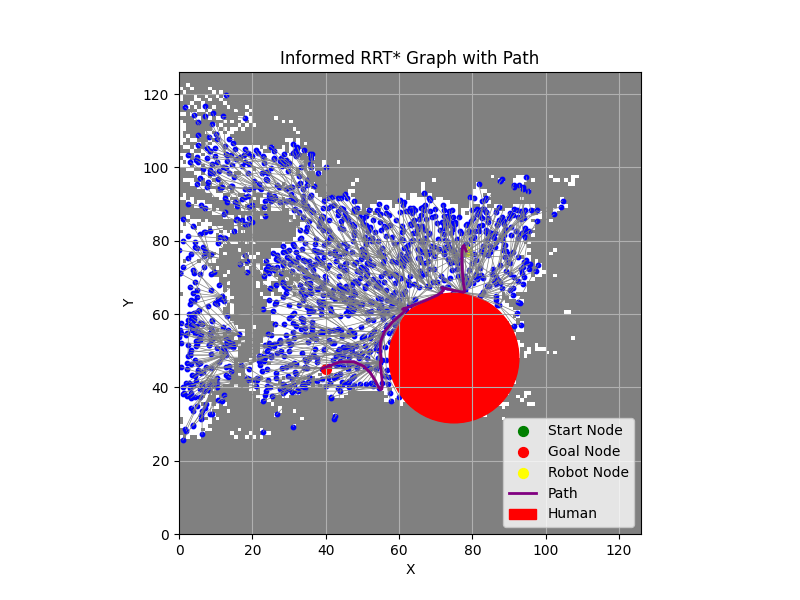
\includegraphics[width=\linewidth, trim={0.0cm 0.0cm 0.0cm 1.9cm}, clip]{Figs/40_45_to_80_80_prox=17.68_back=True.png}
%\caption{$r_{human}=0.893$m}
\end{subfigure} 
\begin{subfigure}{0.8\linewidth}
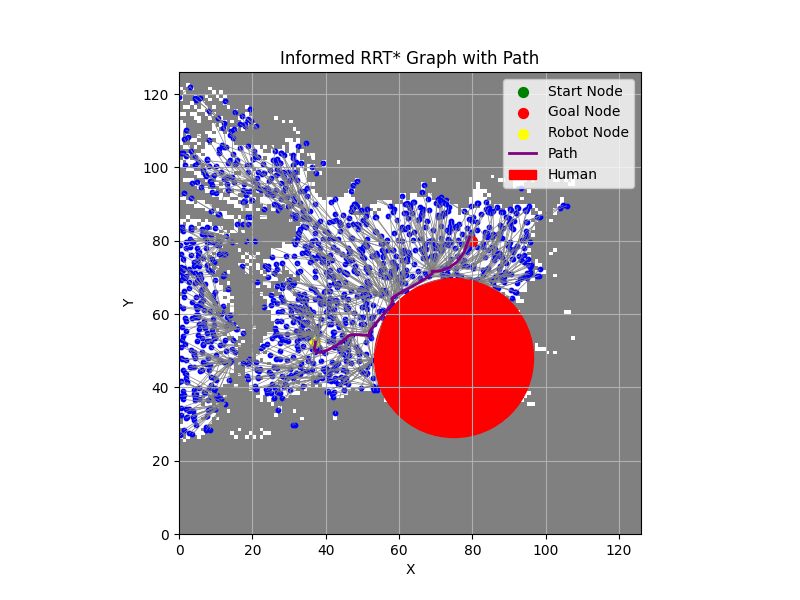
\includegraphics[width=\linewidth, trim={0.0cm 0.0cm 0.0cm 1.9cm}, clip]{Figs/40_45_to_80_80_prox=21.68_back=False.png}
%\caption{$r_{human}=1.084$m}
\end{subfigure} 
\caption{Navigation results using our RRT* inspired algorithm, using radii $r_{human}\in\{0.893m, 1.084m\}$.}
\label{ch6:fig:path_res}
\end{figure}

The navigation module is based on a sampling-based planner inspired by the RRT* (Rapidly-exploring Random Tree Star) algorithm~\citep{karaman2011sampling}. The implementation retains the core structure of RRT*, including incremental tree expansion, nearest-neighbor selection, and local rewiring, but modifies both the sampling strategy and cost function to incorporate social constraints. As a result, the classical guarantees of probabilistic completeness and asymptotic optimality do not strictly apply, and the method is interpreted as an RRT*-inspired heuristic.

After an initial phase of uniform exploration to obtain a feasible solution, the search is biased toward an informed region of the state space analogous to Informed RRT*. In its ideal formulation, this region is defined as the prolate hyperspheroid:

\[
\mathcal{X}_{\text{sub}} =
\left\{
z \in \mathcal{X} \;\middle|\;
\|z - z_{\text{start}}\|_2 + \|z - z_{\text{goal}}\|_2 \leq c_{\text{best}}
\right\},
\]

where $c_{\text{best}}$ is the cost of the best solution found so far. In the present implementation, this bias is approximated via rejection sampling over the full configuration space rather than direct sampling from $\mathcal{X}_{\text{sub}}$.

Social constraints are encoded through a human-aware cost function. Humans are modeled as circular regions with interaction radii derived from proxemic theory. The incremental cost of extending a node $z_{\text{new}}$ is defined as:

\[
C(z_{\text{new}}) = C(z_{\text{parent}}) + d(z_{\text{parent}}, z_{\text{new}}) + \alpha \sum_{h \in H} P(z_{\text{new}}, h),
\]

where $d(\cdot)$ denotes Euclidean edge cost, $\alpha$ is a weighting factor, and $P(\cdot)$ is a proxemic penalty enforcing socially acceptable distances and collision avoidance.

In our context, the penalty from the human is defined as the following piece-wise function.

$$
P(z_{\text{new}}, h) = \begin{cases} 
\infty & \text{if } 0 \le d < r_h \\ 
(d - r_h)^2 & \text{otherwise}
\end{cases}
$$

The distance $d$ denotes the Euclidean distance from the human, and $r_h$ represents the human’s proxemic radius. This penalty term enforces that trajectory samples remain outside the human’s proxemic region while encouraging the robot to stay close to, but not violate, the boundary defined by $r_h$.

Since $r_h$ is a cultural parameter, it directly influences trajectory planning: larger values of $r_h$ cause the robot to maintain greater distances from humans, whereas smaller values allow it to pass closer.
When the Cultural Adapter modifies this value in the Adaptation (A) paradigm, the path-planning pipeline is retriggered using the robot’s current localization. The destination is set to point B if it has not yet been reached, or to point A if the robot is already returning after reaching B.
In the other paradigms, namely Baseline (B) and Foreknowledge (F), $r_h$ remains static. Consequently, planning is triggered only twice: initially from point A to point B, and after reaching point B, for the return path from point B to point A. %\color{red} Continuo quindi a non capire i 3 segmenti di cui parli nella conversation. Bisogna fare affetrmazioni non ambigue.
%\color{black}

The final path is smoothed using cubic spline interpolation (\texttt{CubicSpline}), producing a continuous trajectory $S(t)$ suitable for execution, at the cost of deviating from the discrete optimality assumptions of RRT*-style planners.

Trajectory execution on the Pepper platform is performed via sequential waypoint tracking using the GoTo primitive in the Pepper 1.8 SDK. To mitigate stop-and-go behavior induced by waypoint discretization, a runtime filtering strategy is applied that skips intermediate waypoints when sufficiently close to the current target, improving motion continuity.


\subsection{Orchestration and REST API}

The server-side architecture is implemented as a Flask-based REST service that serves as the central orchestration layer for both navigation and dialogue subsystems. It mediates communication between the Pepper robot controller and computational modules responsible for path planning, state estimation, and language-based interaction.

The system is structured as a modular, state-synchronized pipeline in which navigation and interaction processes run concurrently while sharing a unified representation of the robot state. The server maintains an asynchronous estimate of the robot pose $(x, y, \theta)$, received from Pepper’s native localization system via the REST interface. This ensures consistency between the physical platform and the server-side state used for planning and control.

To connect discrete map representations with continuous motion, the system implements bidirectional coordinate transformations between occupancy-grid coordinates and metric world coordinates. These transformations account for map resolution, origin offsets, and axis conventions, ensuring consistent interpretation of spatial information across planning and execution.

The REST interface exposes endpoints for localization updates, dialogue state updates, and trajectory generation. A dedicated endpoint triggers the path-planning pipeline, which is based on a sampling-based strategy inspired by the RRT* (Rapidly-exploring Random Tree Star) framework. The planner combines static obstacle information from the occupancy grid with dynamic cost terms derived from proxemic constraints provided by the dialogue subsystem.

The dialogue subsystem (Conversation Manager) acts as an external state generator that conditions navigation through updates to proxemic parameters. When a change in cultural or interpersonal preferences is detected, the corresponding proxemic radius is updated on the server. This triggers a validation step that checks whether the current trajectory remains feasible under the updated social constraints. If violated, replanning is initiated using the updated cost function, ensuring consistency between motion plans and the current interaction context.

Communication between modules is implemented via JSON-based payloads exchanged through the REST interface. This design decouples dialogue interpretation, state management, and motion planning while maintaining runtime coupling through shared state synchronization.

%\color{red}Da qui in poi stai parlando di protocollo per esperimenti, non è più una descrizione del sistema. Da qualche parte nel prossimo capitolo andranno 
%\color{black}

%\color{red}


%\color{black}
